\makeatletter
%\newcommand{\rmnum}[1]{\romannumeral #1 }
%\newcommand{\Rmnum}[1]{\expandafter\@slowromancap\romannumeral #1@}
\makeatother
\ifpdf
\graphicspath{{Chapter3/Chapter3Figs/PNG/}{Chapter3/Chapter3Figs/PDF/}{Chapter3/Chapter3Figs/}}
\else
\graphicspath{{Chapter3/Chapter3Figs/EPS/}{Chapter3/Chapter3Figs/}}
\fi

\chapter{BERI Multiprocessor Architecture}
	\label{chapter_methadology}

\section{BERI Architecture}
	The Bluespec Extensible RISC Implementation (BERI) processor is based on a 64-bit MIPS ISA. The processor is implemented in Bluespec SystemVerilog. The initial implementation was done by Gregory Chadwick \cite{Chadwick12,Chadwick13} and extended to support MIPS R4000 \cite{MIPS} by Jonathan Woodruff \cite{jon_thesis} and others \cite{BERITech_0,BERITech_1}.
	
	This processor has been developed as part of the CTSRD \& MRC2 projects \cite{CTSRD,MRC2}, hence, it is a good base platform for multiprocessor research and development. The team is also actively advancing the testing environment, model checking tools, compiler support and the operating system; ideal for hardware development and evaluation.
	
	BERI is a single issue, in-order processor with 6 pipeline stages. It has a branch predictor and register renaming. The memory structure consists of level 1 (L1) instruction and data caches, and a shared level 2 (L2) cache. 
	BERI with capability support is known as Capability Hardware Enhanced RISC Instructions (CHERI) \cite{Woodruff14,Watson12,Watson15}. 
	Figure \ref{beri_pipeline} shows a logical layout of the processor pipeline, control logic, and memory subsystem. 
	All variations of this processor can be synthesised to run on a Field Programmable Gate Array (FPGA) device.
	

	
	\paragraph{Pipeline Stages}	
		\begin{enumerate}
			\item Instruction Fetch: The program counter is used to request an instruction from memory.
			\item Scheduler: This stage is an optimisation, designed to access the register file and the branch predictor. 
			\item Decode: Instruction behaviour is identified.
			\item Execute: Arithmetic or assignment operations are performed at this stage.
			\item Memory Access: This pipeline stage communicates with memory through the data cache.
			\item Writeback: Any updates to the overall state are committed.
		\end{enumerate}

	\begin{figure}[t]
		\centering 
			\makebox{\includegraphics[width=0.97\textwidth,height=\textheight,keepaspectratio]{BERI_pipeline}}
			\caption{BERI processor architecture} 
			\label{beri_pipeline}
	\end{figure}

	\paragraph{Memory System}
		\begin{itemize}
			\item Instruction Cache: This L1 cache is designed to hold instructions and only performs loads.
			\item Data Cache: This L1 cache loads and stores data.
			\item L2 Cache: A shared cache responsible for holding both instructions and data.
			\item AXI Bus: A standard memory communication interface.
		\end{itemize}
		
	\paragraph{Peripherals}
		\begin{itemize}
			\item Boot ROM: Holds the memory contents required to boot the processor.
			\item Debug Unit: This device is used to inject instructions into the processor pipeline. The instructions can modify general purpose registers and memory. 
			\item PIC: The Programmable Interrupt Controller (PIC) multiplexes external interrupts.
		\end{itemize}
	
\section{Bluespec System Verilog}
	Traditional hardware description languages such as System Verilog have been widely used for hardware development. To aid productivity our research team has been exploiting a higher-level HDL, Bluespec System Verilog (BSV) \cite{bluespec,richards10} is a language initially developed at the Massachusetts Institute of Technology that allows extensible hardware design development. It is currently a property of Bluespec Inc. \cite{BSVREF}. 
	
	BSV adds a much needed level of abstraction to System Verilog, a rich type system, and flow control. The BSV language, together with the BSC compiler generate synthesisable Verilog RTL or SystemC. BSV retains some of the structure and syntax of System Verilog but also adds some Haskell syntax, improving the language extensibility.
	
	Bluespec designs synthesised into SystemC can be simulated using Bluesim to produce a cycle accurate model. Some tests and results presented in this dissertation are based on Bluesim output. The simulator has proven to be an excellent tool for testing and debugging our processor designs. Additionally, the produced results closely match hardware behaviour, making it an invaluable tool.

\section{Multiprocessor BERI Design}
	I have extended the BERI processor core into a multi-core design. Multi-core BERI supports a large number of cores; the design complexity and size is limited by the Bluespec compiler synthesis time, FPGA area, and the shared memory design. Most of the work described in this dissertation is based on a dual-core BERI, however multi-core version with up to 12 cores have been tested in simulation. Due to FPGA size limitations, the hardware tests have been limited to 1-4 cores on Altera DE-4 Stratix-4 \cite{TerasicDE4}; larger FPGAs should be able to support more cores.

	BERI multi-core is a shared memory multiprocessor. The private L1 caches of each BERI core (I-Cache and D-Cache) communicate with a single shared L2 cache. Numerous pipeline modifications were made in order to support multiple cores. The performance of larger designs will be limited by the shared L2 cache and communication interfaces. Several memory coherence models have been tested as a part of this research, I discuss two in this dissertation, directory coherence and time-based coherence, justified in Chapter \ref{chapter_background}. 
	
	\subsection{Memory Modification}
		\paragraph{Directory Coherence} The directory is contained within the L2 cache (Figure \ref{beri_directory}). If the directory identifies memory sharing and chooses to invalidate a privately cached line, it sends a message through a dedicated coherence interface. The message is processed by a coherence module which selects recipients based on the list of sharers. This ensures no coherence congestion on the shared bus and fast invalidate delivery. 
		
		\begin{figure}[t]
			\centering 
				\makebox{\includegraphics[width=\textwidth,height=\textheight,keepaspectratio]{BERI_directory}}
				\caption{BERI dual-core processor, directory-based coherence} 
				\label{beri_directory}
		\end{figure}
		
		\paragraph{Time-Based Coherence} This coherence scheme operates from within the private caches, performing self-invalidation (Figure \ref{beri_timebased}). As a result, the L2 cache is stock and no coherence module or network is required.
		
		\begin{figure}[t]
			\centering 
				\makebox{\includegraphics[width=\textwidth,height=\textheight,keepaspectratio]{BERI_timebased}}
				\caption{BERI dual-core processor, time-based coherence}
				\label{beri_timebased}
		\end{figure}


	\subsection{Core Identification}
		Software often requires a method for identifying individual processor cores. The operating system learns the hardware set up and uses this information to schedule software threads. Core identification is accomplished though a special coprocessor 0 (CP0) instruction. The mechanism used in BERI is similar to MIPS processors \cite{MIPS}. The ID is accessible in kernel-space and returns a 32 bit value. The bottom 16 bits hold the core id and the top 16 bits contain the total core count \{0 = One Core\}.
		%(Figure \ref{core_id}). 
		The distribution of core identifiers occurs at Bluespec compile time. Once built, the identifiers are fixed and cannot be changed or overwritten. 
		%This register is accessed during the FreeBSD boot procedure.

		\begin{comment}
		\begin{figure}[!h]
		\centering
			\newcommand{\colorbitbox}[3]{%
			\rlap{\bitbox{#2}{\color{#1}\rule{\width}{\height}}}%
			\bitbox{#2}{#3}}
			\definecolor{lightcyan}{rgb}{0.6,1,1}
			\definecolor{lightgreen}{rgb}{0.7,1,0.7}
			\begin{bytefield}[bitheight=\widthof{~Valid~},bitwidth=\widthof{\large x~},
			boxformatting={\centering\small}]{32}
			\bitheader[endianness=big]{31,16,15,0} \\
			\colorbitbox{lightgreen}{16}{Total Core Count} &
			\colorbitbox{lightcyan}{16}{Individual Core ID} &
			\end{bytefield}
			\caption{BERI Core Identification} 
			\label{core_id}
		\end{figure}
		%\vspace{-5mm}
		\end{comment}
		
	\subsection{Interrupt Delivery}
		In commercial multiprocessors, interrupts are often serviced through a hierarchy of programmable interrupt controllers (PIC's). The master PIC distributes interrupts to PIC's further down the hierarchy. The original PIC for single-core BERI was developed by Robert Norton \cite{Norton15}. BERI multi-core requires one PIC per core. The hierarchy is flat and interrupts are delivered to the PIC's simultaneously. Individual PIC's decide whether an interrupt should be reported to the given core.

	\subsection{Load Linked and Store Conditional}
		The correct implementation of synchronisation Load-Linked (LL) and Store Conditional (SC) instructions is critical for correct multiprocessor operation.
		The pair of instructions is frequently used in multithreading to achieve synchronisation. LL acts much like a typical load instruction and returns data from memory, an SC to the same memory location will only store data if no other updates have occurred since the LL. The SC instruction is expected to return a response, success or failure. 
		
		The behaviour of LL and SC operations is implementation and ISA dependent. The constrained ISA specification can be exploited by hardware designers for optimising the LL/SC scheme. The BERI multiprocessor LL/SC protocol is based around the MIPS specification \cite{MIPS}, and all multiprocessor versions use this design. The protocol is illustrated in Figure \ref{beri_llsc}.
		
		\begin{figure}[!t]
			\centering 
				\makebox{\includegraphics[trim={0 2.9cm 0 3cm},clip,width=\textwidth,height=\textheight,keepaspectratio]{BERI_llsc}}
				\caption{BERI LL/SC mechanism} 
				\label{beri_llsc}
		\end{figure}
		%\vspace{-5mm}

		Significant differences in the coherence schemes have necessitated a generalised LL/SC design. In order to avoid any memory consistency issues, all memory locations are propagated directly to the shared L2 cache. This ensures up-to-date data observations. This scheme adds latency overheads, however, a relatively low occurrence of LL and SC instructions and expected losses due to synchronisation, permit this implementation.
		
		The L2 cache holds one LL/SC register per core interface, the MIPS specification does not expect more than one LL operation at a time. An LL is treated as a miss in the private L1 data cache. If an SC hits in the private cache, the memory location is invalidated and the SC is written through into the L2. The pipeline expects a success or fail for each SC operation and unlike normal stores, the L2 returns a success flag to the L1.
		
		In addition to LL/SC, software often uses other synchronisation mechanisms such as the MIPS SYNC instruction. Unlike LL/SC, the behaviour of SYNC instructions is more dependent on the memory consistency model.

\section{FPGA Implementation}
	\label{fpga_implementation}
	The BERI processor and its variants can be synthesised for an FPGA. We use the Terasic DE4 board equipped with a Stratix-4 FPGA. The board includes dual DDR2 sockets, USB (debugging and testing via JTAG), PCI-E, Gigabit Ethernet, SD-Card support (used for file transfer), SATA, and other interfaces.
	
	\begin{figure}
	\setlength{\fboxsep}{0pt}%
	\setlength{\fboxrule}{1pt}%
	%\setlength{\fboxrule}{0pt}%
	
		\vspace{-6mm}
		\begin{subfigure}[b]{1\linewidth}
		\centering
		\includegraphics[width=0.92\linewidth]{quartus_dualcore_legend}
		%\caption{Core Pipelines} 
		%\label{dualcore_quartus:b} 
		%\vspace{4ex}
		\end{subfigure} 
		\vspace{-2mm}

\begin{comment}
		\begin{subfigure}[b]{1\linewidth}
		\centering
		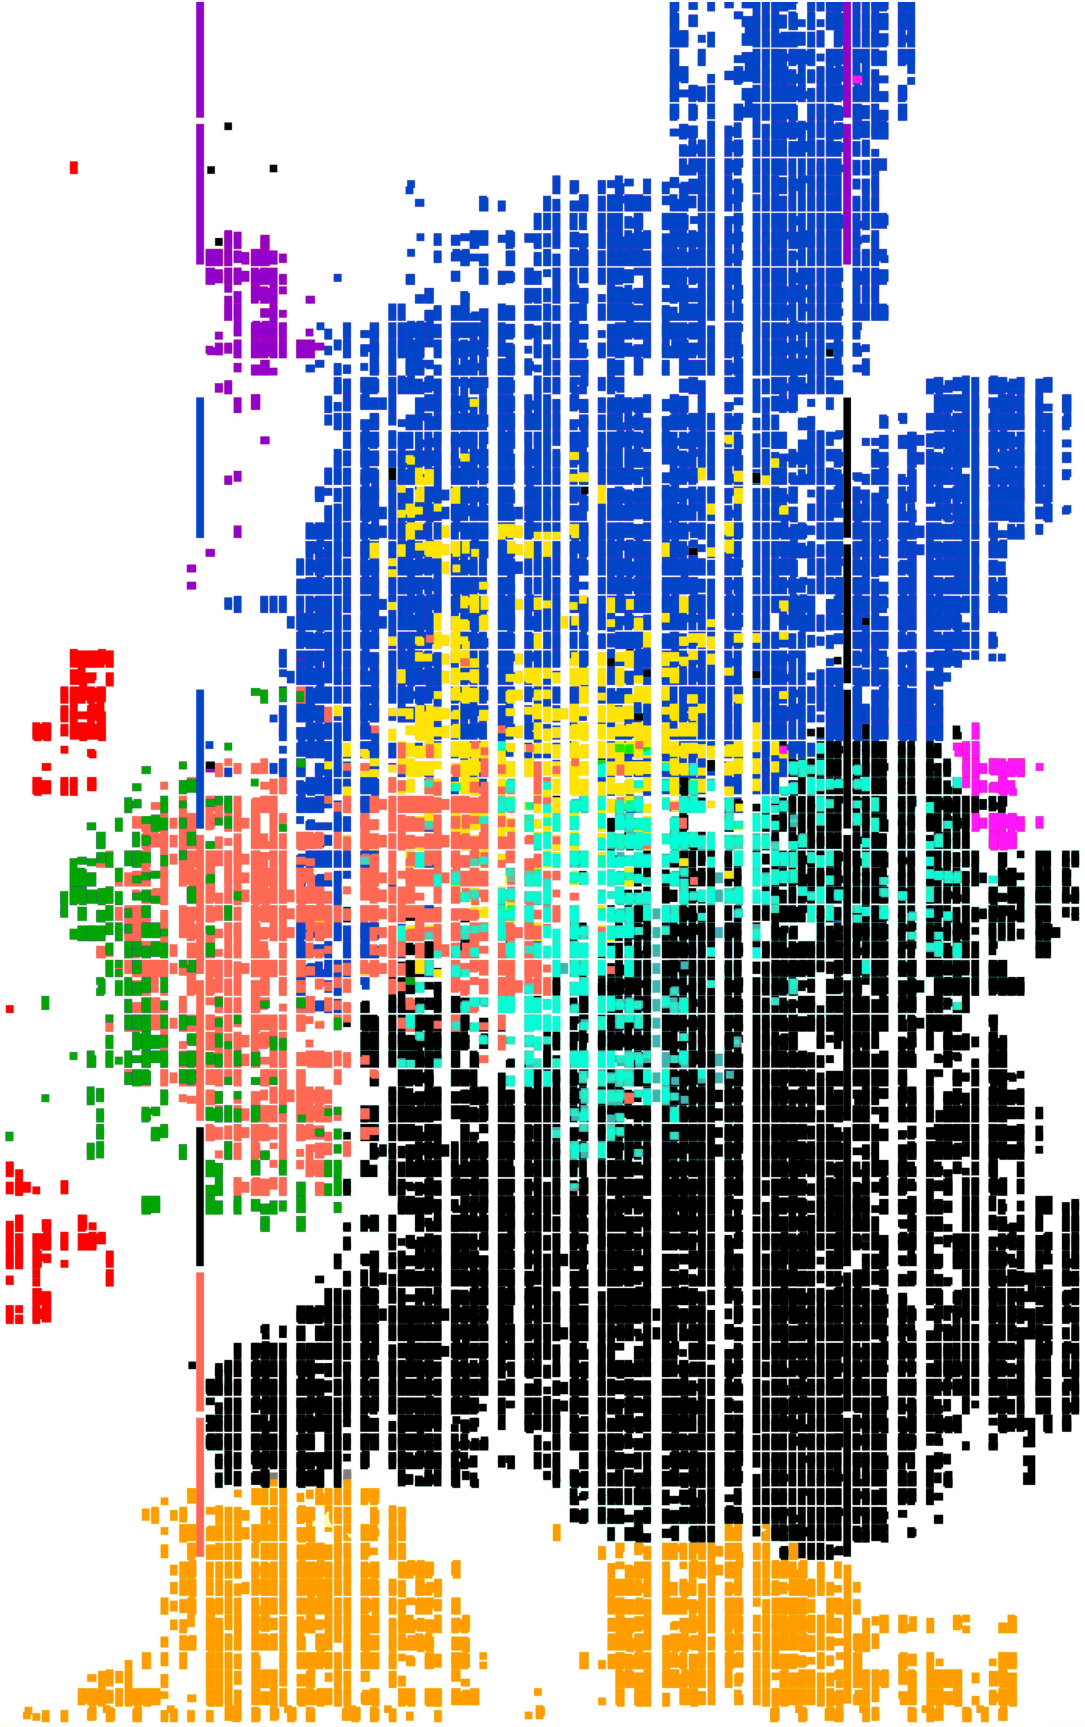
\includegraphics[width=0.83\linewidth]{quartus_dualcore_full}
		\vspace{4ex}
		\end{subfigure}%% 
		\caption{Quartus Dual-Core FPGA Layout}
		\label{dualcore_quartus_full}
\end{comment}
		
%\begin{comment}
		\begin{subfigure}[b]{0.5\linewidth}
		\centering
		\fbox{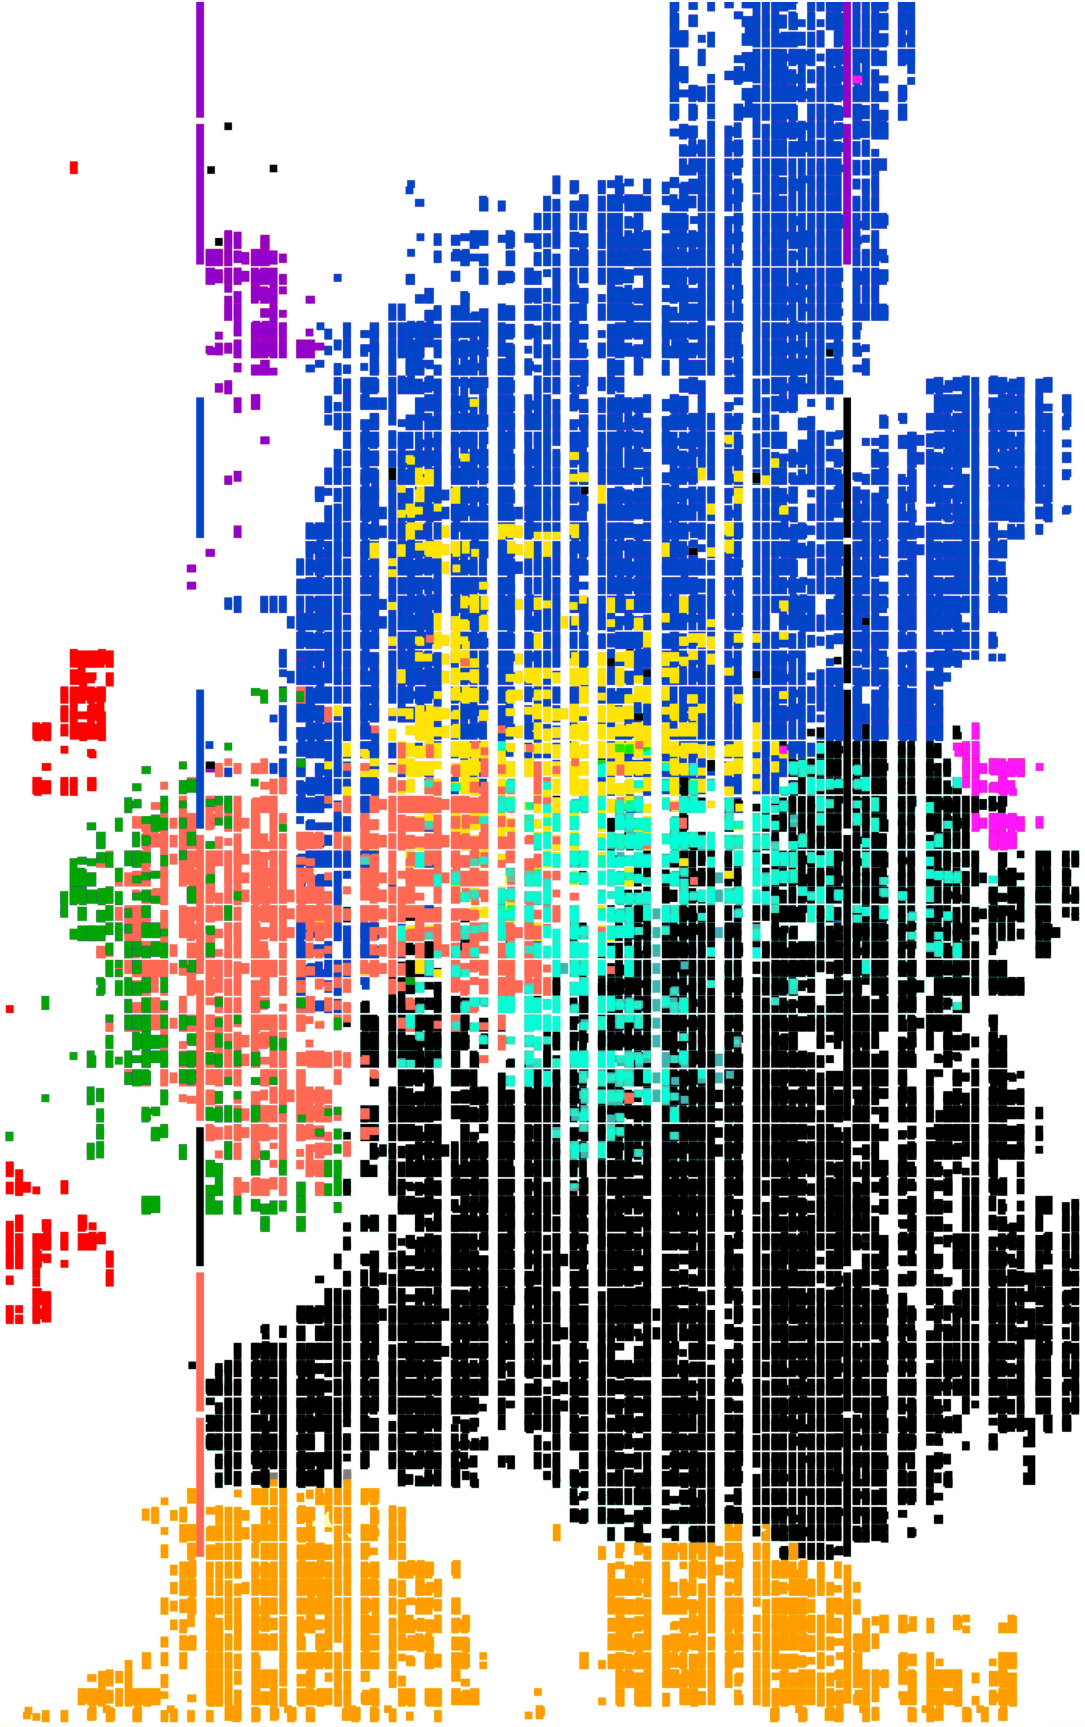
\includegraphics[width=0.83\linewidth]{quartus_dualcore_full}}
		\caption{Complete design} 
		\label{dualcore_quartus:a} 
		\vspace{4ex}
		\end{subfigure}%% 
		\begin{subfigure}[b]{0.5\linewidth}
		\centering
		\fbox{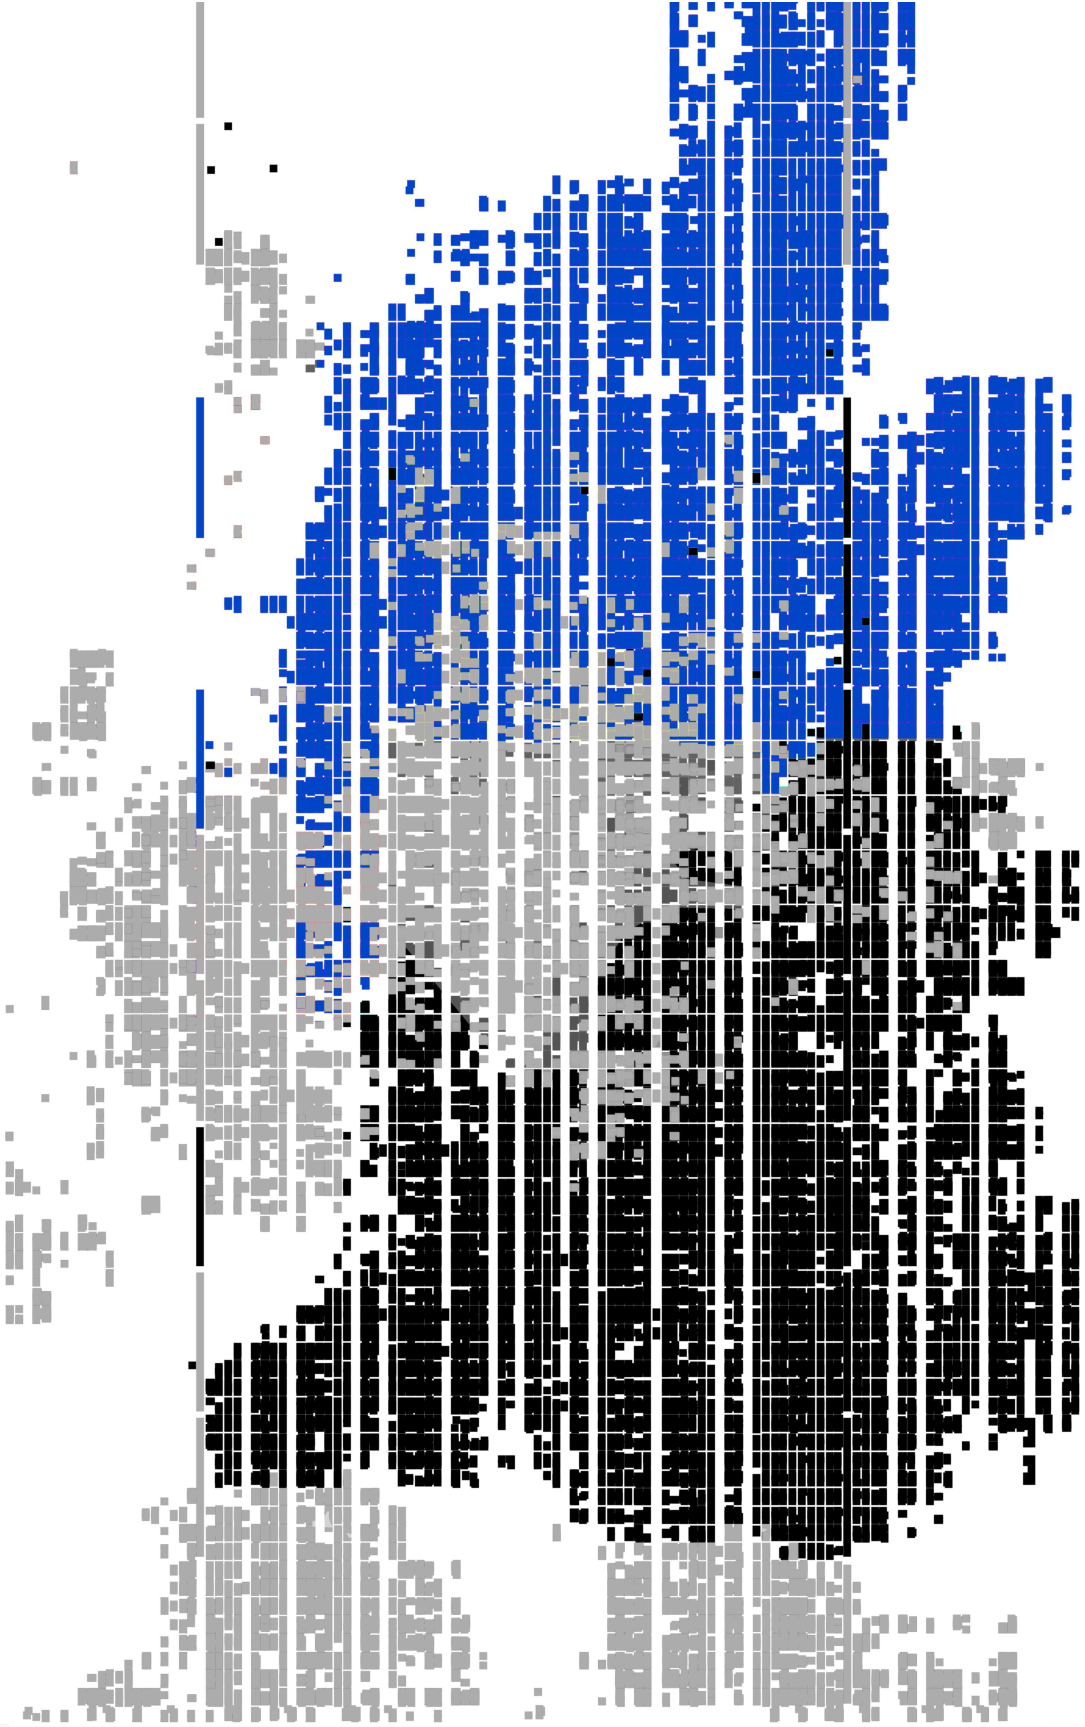
\includegraphics[width=0.83\linewidth]{quartus_dualcore_cores}}
		\caption{Two processor pipelines} 
		\label{dualcore_quartus:b} 
		\vspace{4ex}
		\end{subfigure}
		\begin{subfigure}[b]{0.5\linewidth}
		\centering
		\fbox{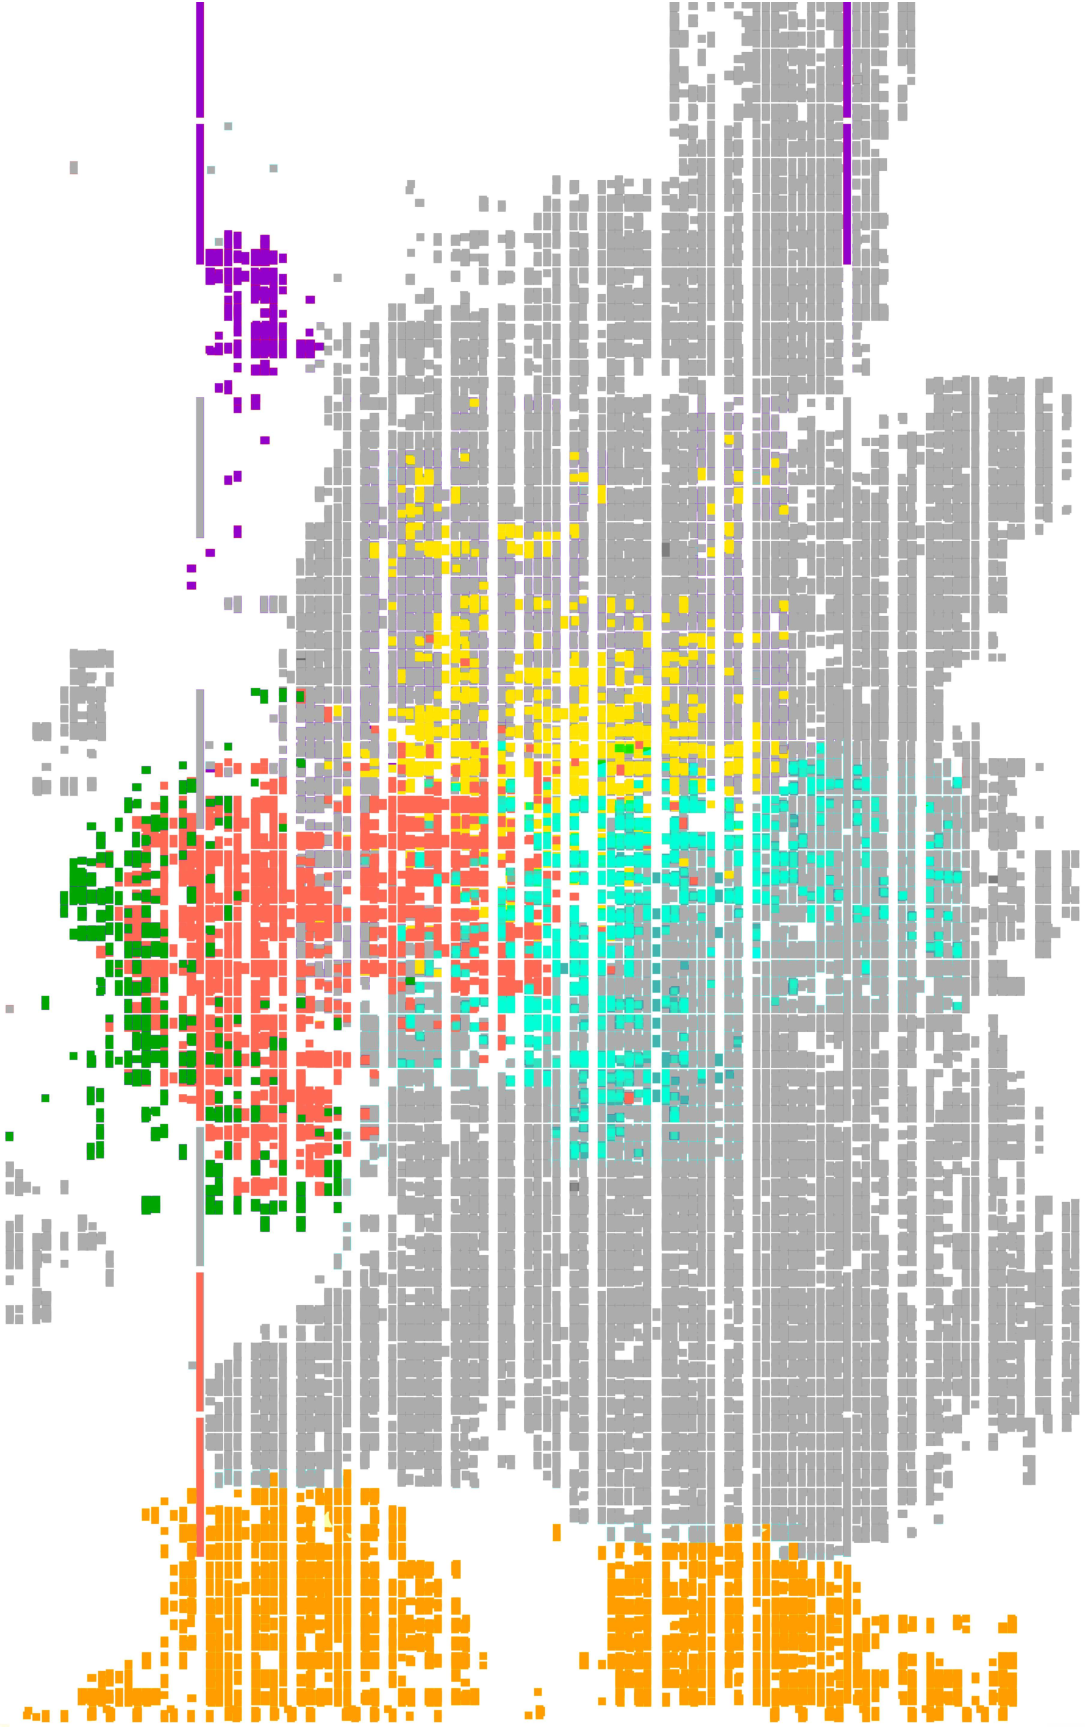
\includegraphics[width=0.83\linewidth]{quartus_dualcore_memory}}
		\caption{Memory hierarchy} 
		\label{dualcore_quartus:c} 
		\end{subfigure}%%
		\begin{subfigure}[b]{0.5\linewidth}
		\centering
		\fbox{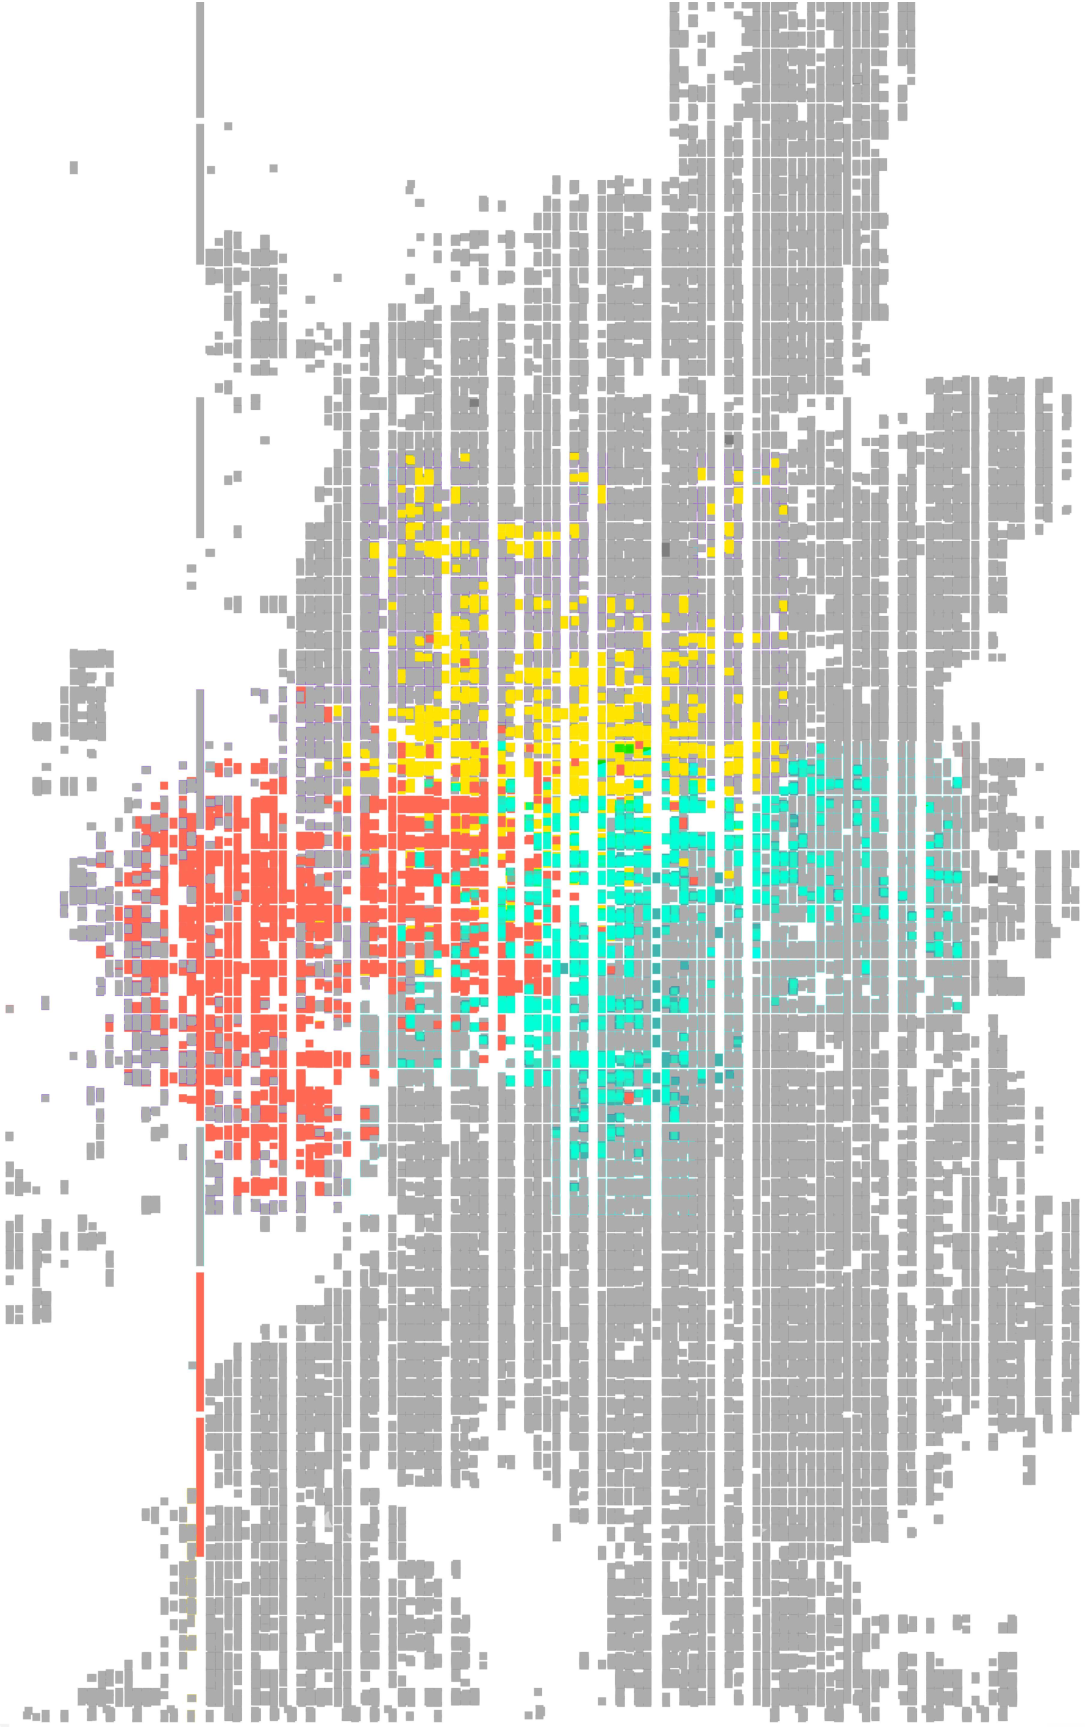
\includegraphics[width=0.83\linewidth]{quartus_dualcore_caches}}
		\caption{Cache hierarchy} 
		\label{dualcore_quartus:d} 
		\end{subfigure} 
		\caption{Dual-core BERI, Quartus FPGA layout}
		\label{dualcore_quartus}
%\end{comment}
	\end{figure}

\begin{comment}	
	\begin{figure}[!h]
		\centering 
			\makebox{\includegraphics[width=\textwidth,height=\textheight,keepaspectratio]{dualcore_fpga}}
			\caption{Dual-Core BERI FPGA Layout} \label{dualcore_fpga}
	\end{figure}
\end{comment}

	The Bluespec compiler can produce verilog which is synthesizable through the Altera Quartus tools. Figure \ref{dualcore_quartus} shows the Quartus synthesised layout of the BERI dual-core processor. Due to the visualisation features of Quartus, some architectural components are overlaid and may not be correctly scaled. Specifics of the coherence mechanism are difficult to differentiate in the layout tool, and look almost identical. The images shown have been generated from a directory design.
	
	\begin{description}
		\item[(a)] Layout of dual-core BERI components: two BERI pipelines, two private data caches (D-Cache's), shared level 2 cache, DRAM controller, boot memory, AXI bus interface, two UARTs, and the debug units. It is not possible to highlight the PIC's as they mostly consist of wiring and minimal logic. The L1 data caches appear larger than normal, as they communicate with the TLB, pipeline stages, and other processor components. As a result the cache logic is spread over a large portion of the FPGA.
		\item[(b)] Two processor pipelines. The L1 instruction caches are included in the highlighted regions.
		\item[(c)] The memory, hierarchy and interconnect are visible in this image. The memory merge unit is not visible, located within the overlapping L1 and L2 logic regions.
		\item[(d)] Two L1 caches and the shared L2 are shown. 
	\end{description}
	
	All the multiprocessor versions of BERI used in this dissertation operate at 100MHz. The DRAM module operates at 200MHz and typically has a capacity of 1GB. BERI dual-core directory version utilizes approximately 58\% of the FPGA logic, with the time-based version requiring around 57\%.

%\clearpage
\section{Testing and Debugging}
	A range of test frameworks have been developed for the BERI project by a large number of people including Robert Watson, Simon Moore, Jonathan Woodruff, Michael Roe, Brooks Davis, David Chisnall, Alexandre Joannou, Theo Markettos, Robert Norton, Colin Rothwell, Stacey Son, Steven Murdoch, Nirav Dave, Matthew Naylor, and myself (Members of the CTSRD project \cite{ctsrd15}). Most of these tests have been used to validate the architectural properties of our system.

	\subsection{Hardware and Software Tracing}
		BSV provides display statements, equivalent to C language print. These statements are used for tracing and debugging when using Bluesim. The tracing technique is used by the Cheritest suite, AXE tests, and bare metal tests in simulation.
		
		Tracing and debugging in hardware is done through a dedicated debug unit, one per core. The debug unit injects instructions into the processor pipeline. These instructions are independent but may cause side-effects, as they are permitted to modify registers and memory. This module also maintains a trace buffer which can be used to log instructions in hardware.
	
	\subsection{Cheritest}
		This test suite is included in the BERI open-source project. There are over 2000 tests currently in the suite, ranging from basic arithmetic, to TLB operations and exception handling. The suite has been constructed by Robert Watson, Michael Roe, Stephen Murdoch, with test contributions from a number of CTSRD \& MRC2 project members \cite{CTSRD,MRC2}. I have added a range of tests for multi-core versions of the processor. This suite has been a critical part of the processor development.
		
		Processor models are regularly tested and verified through the Jenkins continuous integration framework. This automatic tool is currently generating Bluesim designs evaluated through Cheritest, as well as Quartus synthesised FPGA files.
		
	\subsection{Bare Metal Tests}
		In addition to Cheritest suite, we also use a set of bare metal, C language-based tests. Tests are compiled with GCC for MIPS 64-bit architectures. These tests allow us to check software compatibility without the need of an OS or hardware. They can also be loaded into an FPGA design. Some results obtained in Chapter \ref{chapter_validation} and \ref{chapter_sca} are based around the bare metal framework. 
		%Table \ref{vaucher_system_info} shows details of the testing environment. 
		Bare metal tests simulated through Bluesim are cycle accurate; underlying hardware characteristics should not affect the outcome. 

	\subsection{CHERI Litmus Tests}
		Litmus tests are discussed in detail in Chapter \ref{chapter_validation}. They are short tests, usually limited to a small number of instructions, designed to discern the memory consistency model of a given architecture. The CHERI Litmus tests \cite{CHERI_litmus} are designed to run bare metal on BERI/CHERI. These tests have been used to analyse the behaviour of the coherence schemes described in this dissertation.
		
	\subsection{Memory Consistency Checker}
		The AXE checker \cite{AXE_checker,bluecheck}, tests the memory subsystem in isolation and independent of the processor pipeline. Memory can be stressed much more as only memory instructions are repeatedly injected into the cache framework. Even the basic consistency models exhibit vast amounts of non-determinism. The checker tool exhaustively enumerates all behaviour of a set of memory operations. A general-purpose constraint-solver, Yices \cite{Yices15}, is used to check the traces for inconsistencies. These tests also permit a much faster execution and evaluation time. Every coherence model discussed in this dissertation has been verified through the AXE tool, further details are provided in following chapters.

		\begin{table}[b]
		\begin{center}
		\begin{tabular}{|l|l|}
			\hline		
			\multicolumn{2}{|c|}{Operating System} \\
			\hline
			FreeBSD & 11.0-CURRENT \#0 c2208dd(master) \\
			& Mon Dec 15 16:35:59 UTC 2014 \\
			\hline
			\hline		
			\multicolumn{2}{|c|}{Compiler Parameters} \\
			\hline	
			Compiler & clang version 3.6.0 \\
			Target & cheri-unknown-freebsd \\
			Thread model & posix \\
			\hline
		\end{tabular}
		\caption{FreeBSD environment}
		\label{freebsd_info}
		\end{center} 
		\end{table}
		
		\begin{comment}
		Copyright (c) 1992-2014 The FreeBSD Project.
		Copyright (c) 1979, 1980, 1983, 1986, 1988, 1989, 1991, 1992, 1993, 1994
			The Regents of the University of California. All rights reserved.
		FreeBSD is a registered trademark of The FreeBSD Foundation.
		FreeBSD 11.0-CURRENT #0 c2208dd(master): Mon Dec 15 16:35:59 UTC 2014
		\end{comment}

	\subsection{Benchmarks on FreeBSD}
		\label{freebsd_setup}
		FreeBSD is a open source, Unix-like operating system. A version of this OS is supported on BERI, and a capability enhanced version of the OS is supported on CHERI. Benchmarks and other tests based on FreeBSD, described in this dissertation, run on a single user multi-core version of the OS. The Splash-2 benchmark suite, side-channel attack tests, and other software is compiled for FreeBSD using the CHERI LLVM compiler \cite{Chisnall15,Chisnall14} (Table \ref{freebsd_info}).
		
	\section{Summary}
		The existing BERI uniprocessor and test suit have been extended to provide multi-core support, sufficient for a full OS bring up. This can be used on FPGA for performance or in simulation for detailed analysis. Later chapters exploit this framework to explore cache coherency and side-channel effects on complete systems running large-scale benchmarks and applications.
		
		
		
		
		
		
		
		
		
		
		
		
		
		\begin{comment}
				\begin{table}[!h]
				\begin{center}
				\begin{tabular}{|l|l|}
				\hline
				\multicolumn{2}{|c|}{Hardware Parameters} \\
				\hline
				Architecture          & Intel x86--64 \\
				CPUs                  & 32 \\
				%Threads per core      & 2 \\
				%Cores per socket      & 16 \\
				%Vendor ID            & Intel \\
				%CPU MHz               & 1200.000 \\
				%BogoMIPS             & 6585.73 \\
				%L1 cache's            & 32K \\
				%L2 cache              & 256K \\
				%L3 cache              & 25600K \\
				\hline
				\hline		
				\multicolumn{2}{|c|}{Software Parameters} \\
				\hline
				Compiler & mips-linux-gnu-gcc \\ 
				& Debian 4.4.5-8 \\
				Assembler & mips64-as \\
				Linker & mips-linux-gnu-ld \\
				\hline
				\end{tabular}
				\caption{Simulation Environment}
				\label{vaucher_system_info}
				\end{center} 
				\end{table}
				%\vspace{-10mm}
		\end{comment}